% =====================================================================
%  MOSAIC — 전력설비(전주) 산불위험 조기경보 보고서 (서론·본론·결론)
%  사용 모델 수식을 단계별로 구체화한 논문형 .tex
%  컴파일: xelatex report_full.tex  (권장; 한글 kotex)
%          또는  pdflatex report_full.tex  (2회 — 목차/참조 갱신)
%  내용·수식은 pfire/ 소스 구현과 1:1 대응(모듈명을 각주/회색 텍스트로 표기).
% =====================================================================
\documentclass[11pt,a4paper]{article}

\usepackage{kotex}                          % 한글
\usepackage[margin=2.3cm]{geometry}
\usepackage{amsmath,amssymb,amsthm}
\usepackage{graphicx}
\usepackage{booktabs}
\usepackage{caption}
\usepackage{float}
\usepackage{enumitem}
\usepackage{array}
\usepackage{xcolor}
\usepackage[hidelinks]{hyperref}

\graphicspath{{../outputs/figures/}{../outputs/figures/eda/}{../exposure_v2/}}
\captionsetup{font=small,labelfont=bf}

\newcommand{\src}[1]{{\footnotesize\color{gray}\texttt{#1}}}
\newcommand{\R}{\mathbb{R}}
\newcommand{\E}{\mathbb{E}}
\newcommand{\Var}{\mathrm{Var}}
\newcommand{\clip}{\mathrm{clip}}
\setlength{\parskip}{4pt}

\title{\vspace{-1.0cm}\textbf{전력설비(전주) 산불위험 조기경보 시스템}\\[4pt]
\large 물리 혼합전문가(MoE)와 변별 가능한 풍하 노출의 결정 결합 --- \textbf{MOSAIC}\\[6pt]
\normalsize 사용 모델의 수식·데이터·절차 상세 보고서}
\author{\normalsize 2026 날씨 빅데이터 콘테스트 · 주제1(재난안전) — 기상청 / 한국전력공사}
\date{\normalsize 2026-06-23}

\begin{document}
\maketitle

\begin{abstract}
\noindent
강원도 가상 전주 \textbf{1{,}387{,}831개} 각각에 산불 위험/안전 $\{0,1\}$을 판정하는 문제를
다룬다. 정답 라벨이 주어지지 않는 \emph{presence-only(존재만 관측)} 과제이므로, 과거 발화점
928건(강원 925건)은 학습 타깃이 아니라 \emph{검증·임계값 결정의 앵커}로만 쓴다. 핵심 아이디어는
하루치 위험을 \emph{발화 성향}$\times$\emph{확산·노출 취약}$\times$\emph{그날 기상}의 곱
$h=I\!\times\!S\!\times\!W$로 분해하고, 발화 성향 $I$를 영동·회랑(양간지풍)·영서·산간의 4개
\emph{지역 혼합전문가(MoE)}로 추정하는 것이다. 발화원이 조밀한 영동에서 포화되던 풍하 노출은
발화가중 기대도즈 $\cdot$ Anderson 타원 커널 $\cdot$ 격자 국지정규화로 \emph{변별 가능}하게
재설계하여 결정 위험에 확률 OR로 결합했다. 불확실성은 Poisson--Gamma 켤레 사후와 BYM2 공간 CAR
(Laplace 근사)로, 임계값 신뢰도는 \emph{체제별 conformal}로 명목 90\% 커버리지를 보장한다. 공간
블록 교차검증에서 발화점 recall@top-5\%는 랜덤의 약 2배(0.106)이고 무작위-공간 격차$\approx 0$
(낙관 편향 없음), conformal 실측 커버리지는 0.902다. 본 보고서는 이 시스템에 쓰인 \emph{모든 식과
데이터·절차}를 서론--본론--결론 순으로 단계별로 기술한다.
\end{abstract}

\tableofcontents
\vspace{6pt}\hrule

% =====================================================================
\section{서론}
% =====================================================================

\subsection{문제 정의}
산불은 전력설비(전주) 인근에서 발화하거나 그쪽으로 번질 때 대형 재난으로 이어진다.
2019년 고성--속초 산불의 발화원은 \textbf{한전 특고압선 아크}였고, 양양$\sim$간성에 부는 서풍
푄(föhn)인 \textbf{양간지풍}(순간 최대 $20.4\sim27.6$\,m/s)이 이를 대형화시켰다. 본 과제는 강원
전주 $N=1{,}387{,}831$개 각각에 위험/안전 $\{0,1\}$을 매겨 제출하며, 점수는 정량(20\%; 한전
비공개 정답과의 F1)과 정성(80\%; 합리성·분석능력·활용성·창의성·부합성)으로 채점된다.

\subsection{문제를 지배하는 두 제약}
설계 전체를 두 가지가 지배한다.
\begin{enumerate}[leftmargin=1.4em]
\item \textbf{정답 라벨이 없다(presence-only / PU).} 우리가 가진 발화점은 ``불이 난 곳''만 기록한
데이터이며, ``불이 안 난 곳''이 정말 안전한지는 모른다. 이는 생태학의 \emph{종 분포 모델(SDM)}
및 \emph{Positive--Unlabeled(PU) 학습}과 수학적으로 동형이다. 따라서 발화점을 per-pole 학습
라벨로 쓰면 누수(leakage)와 표집편향이 발생한다 $\Rightarrow$ 발화점은 \emph{지역 집계 앵커
\,·\, 검증 \,·\, 임계값}으로만 사용한다.
\item \textbf{점수의 80\%가 정성평가다.} 점수만 좋은 블랙박스가 아니라 \emph{왜 이 전주가 위험한지
항목별로 설명되는} 물리 기반·해석 가능 시스템이어야 한다.
\end{enumerate}

\subsection{접근(MOSAIC)과 기여}
\textbf{MOSAIC} $=$ \emph{M}ixture-of-experts $\cdot$ \emph{S}patial $\cdot$
\emph{A}nchored(presence-only) $\cdot$ \emph{I}gnition-physics $\cdot$ \emph{C}overage.
본 시스템의 기여는 다음과 같다.
\begin{itemize}[leftmargin=1.4em,itemsep=1pt]
\item 위험의 \textbf{물리적 곱셈 분해} $h=I\cdot S\cdot W$로 해석 가능성을 확보(절\ref{sec:decomp}).
\item 발화 메커니즘이 다른 4개 체제를 \textbf{soft 게이트 혼합전문가}로 부분 풀링(절\ref{sec:moe}).
\item 포화되던 OR 노출을 \textbf{변별 가능한 발화가중 기대도즈}(타원 커널 + 국지정규화)로
재설계해 결정에 결합(절\ref{sec:exposure}).
\item 발화 희소성 보정을 위한 \textbf{경험적 베이즈 + BYM2 공간 사후}, 그리고 라벨 없는 환경에서
신뢰도를 보장하는 \textbf{체제별 conformal}(절\ref{sec:posterior}--\ref{sec:eval}).
\end{itemize}

% =====================================================================
\section{본론 I — 데이터}
% =====================================================================
\src{pfire/config.py, pfire/io.py}

모든 입력은 강원도로 한정되며 좌표계는 EPSG:4326(위경도)이다. 거리·확산 계산은 강원 대표 위도
($\mathrm{LAT0}=37.7^\circ$)의 $\cos$ 보정을 쓴 \emph{근사 평면 km} 좌표에서 수행한다. 데이터는
크게 (i)~전주 마스터, (ii)~기상, (iii)~검증 앵커(발화점)로 나뉜다.

\begin{table}[H]
\centering
\caption{사용 데이터 요약. 행수는 전주 마스터가 모두 $N=1{,}387{,}831$.}
\label{tab:data}
\small
\begin{tabular}{p{3.4cm}p{1.6cm}p{8.4cm}}
\toprule
파일 & 행수 & 제공 변수(용도) \\
\midrule
\texttt{pole\_features} & $N$ & 좌표(lon, lat)·고도·\texttt{fwi\_q90}·\texttt{fwi\_high\_danger\_days}·\texttt{yanggan\_days}·연료 \texttt{mu\_flammability}·\texttt{mu\_southness}(발화/기상/연료 피처) \\
\texttt{pole\_power} & $N$ & \texttt{dist\_to\_powerline}, \texttt{dist\_to\_substation}(전력설비 자산 근접) \\
\texttt{pole\_static\_overlay} & $N$ & \texttt{dist\_to\_forest}, \texttt{dist\_to\_road}, 확산취약 사전계산 $S_p$ \\
\texttt{pole\_landcover\_filled} & $N$ & \texttt{lc\_group}(토지피복 7범주; 발화계수 사전치 조회) \\
\texttt{pole\_sgg} & $N$ & 전주$\to$시군 매핑(체제 앵커·검증용, 하드 라벨 아님) \\
\texttt{pole\_fwi\_obs} & $N$ & 관측 기반 전주 보간 FWI 통계(대안 $W$ 소스) \\
\texttt{fwi\_station\_daily} & 377{,}822 & 관측소 일별 FWI/ISI/FFMC/풍속(일별 $W$, 풍속 표집) \\
\texttt{aws\_obs\_daily} & 377{,}822 & 관측소 일별 풍향 \texttt{wd}/풍속(비영동 풍향 표집) \\
\texttt{aws\_stations\_coords} & 109 & 관측소 좌표·고도(최근접 매핑) \\
\texttt{safemap\_positives} & 928 & 과거 발화점(강원 925) — \emph{검증·임계값 앵커 전용} \\
\texttt{admin\_gangwon} & 42 & 행정경계 WKT(체제 매핑·시각화) \\
\bottomrule
\end{tabular}
\end{table}

\paragraph{탐색적 분석(EDA)이 정한 설계 골격.} EDA는 모델 구조를 직접 정당화한다.
\begin{itemize}[leftmargin=1.4em,itemsep=1pt]
\item 발화의 \textbf{91\%가 산림}에서, \textbf{봄(3$\sim$5월) 59\%}에 집중 $\Rightarrow$ 토지피복·산림
거리·시즌(2$\sim$5월)을 핵심 피처/창으로.
\item 불의 \emph{크기}는 발화지형이 아니라 \textbf{바람·ISI(초기확산)}가 좌우(화재당일 풍속
$\rho{=}{+}0.29$, ISI ${+}0.26$) $\Rightarrow$ 일별 ISI/FFMC 동역학과 풍하 확산을 모델에.
\item 기상은 전주 단위가 아니라 $\sim$13\,km \textbf{격자 단위}로 작용(전주$\to$최근접 관측소 중앙값
$4.8$\,km) $\Rightarrow$ $W$는 격자/관측소 해상도.
\item 체제별 신호 분리: 영동 양간일 $2.33$·FWI $9.2$ vs 영서 $0.3$·$5.24$, 케이스-크로스오버 풍속
AUC가 회랑 $0.664$·영동잔여 $0.562$인 반면 영서/산간은 $\approx 0.49$(무변별)
$\Rightarrow$ \emph{지역 혼합전문가}와 \emph{wind-driven 체제에만} 풍하 노출 적용.
\end{itemize}

% =====================================================================
\section{본론 II — 모델: 사용 수식의 단계별 전개}
% =====================================================================

\subsection{기호 약속}
\begin{center}
\small
\begin{tabular}{ll}
\toprule
기호 & 의미 \\
\midrule
$p$ & 전주 인덱스($N=1{,}387{,}831$) \\
$t$ & 날짜(산불조심기간 2$\sim$5월) \\
$r$ & 체제: 영동(yeongdong)·회랑(corridor)·영서(yeongseo)·산간(mountain) \\
$g(p)$ & 전주 $p$가 속한 기상 격자($\sim$13\,km) \\
$I,S,W\in[0,1]$ & 발화 성향 / 확산·노출 취약 / 기상 위험 \\
$h,R\in[0,1]$ & 일 위험 / 시즌 위험 \\
$y_g,\,n_g$ & 지역 $g$의 발화수(앵커) / 전주수(노출) \\
\bottomrule
\end{tabular}
\end{center}
모든 성분은 $[0,1]$로 정규화하며 NaN·범위를 강제 검증한다(\src{hazard.\_validate\_unit}).

% ---------------------------------------------------------------
\subsection{1단계 — 위험의 곱셈 분해}\label{sec:decomp}
% ---------------------------------------------------------------
\src{pfire/hazard.py}

전주 하루치 위험을 세 항의 곱으로 본다:
\begin{equation}
h(p,t)\;=\;\underbrace{I(p)}_{\text{발화 성향}}\;\times\;
\underbrace{S(p)}_{\text{확산·노출 취약}}\;\times\;
\underbrace{W(g(p),t)}_{\text{그날 기상}}\ \in[0,1].
\label{eq:hazard}
\end{equation}
\textbf{왜 곱인가.} 셋 중 하나라도 0이면 위험 0이라는 \emph{AND} 성격이 물리적으로 타당하다(불씨가
없거나, 탈 게 없거나, 날이 궂지 않으면 안 난다). 또한 각 항을 따로 해석해 ``왜 위험한가''를
항목별로 설명할 수 있다.

\textbf{시즌 집계 $R(p)$.} 산불조심기간 $T$일을 하나의 시즌 위험으로 모은다. $W$가 단일 시즌통계면
MVP 경로로 $R=I\,S\,W$이고, 일별 $W_t$가 주어지면 \emph{기하평균}(로그합 평균)으로 집계해 한 번의
고위험일이 시즌 위험을 폭주시키는 것을 완화한다:
\begin{align}
\text{(MVP)}\quad & R(p)=I(p)\,S(p)\,W(p),\\
\text{(일별)}\quad & R(p)=\exp\!\Big(\tfrac{1}{T}\textstyle\sum_{t=1}^{T}
\log\big[\clip(I\,S\,W_t,\,\varepsilon,1)\big]\Big),\qquad \varepsilon=10^{-9}.
\label{eq:season}
\end{align}

% ---------------------------------------------------------------
\subsection{2단계 — 발화 성향 $I(p)$: 지역 혼합전문가(MoE)}\label{sec:moe}
% ---------------------------------------------------------------
\src{pfire/experts.py, pfire/regimes.py, pfire/config.py}

체제별로 발화 메커니즘이 다르다(영동=가뭄·FWI, 회랑=양간풍·송전선, 영서=도로·입산자,
산간=연료·산림). 전 지역 단일 모델은 평균에 묻히고, 지역별 개별 모델은 데이터가 쪼개져
과적합한다. 그 중간(\emph{부분 풀링})을 soft 게이트 혼합전문가로 구현한다. 절차는 네 단계다.

\paragraph{(2a) 피처 정규화 — 모두 $[0,1]$, 클수록 위험.}
거리 피처는 \emph{가까울수록 위험}이므로 지수 감쇠로 정규화한다:
\begin{equation}
\mathrm{feat}_{\text{dist}}(p)=\exp\!\big(-\,d(p)/\text{scale}\big),\qquad
\text{scale}=\begin{cases}
100\,\text{m} & \text{산림(forest)}\\
300\,\text{m} & \text{도로(road)}\\
1500\,\text{m} & \text{송전선(powerline)}\\
3000\,\text{m} & \text{변전소(substation, 선택)}
\end{cases}
\label{eq:decay}
\end{equation}
나머지 피처: FWI(\texttt{fwi\_q90})·양간일(\texttt{yanggan\_days})은 min--max 정규화, 연료는
$\clip(\mu_{\text{flam}},0,1)$, 토지피복은 도메인 사전치 조회
\begin{equation}
\mathrm{landcover}(p)=\mathrm{lc\_ignition}\big(\mathrm{lc\_group}(p)\big),\quad
\mathrm{lc\_ignition}:\{\text{산림}{\to}1.00,\ \text{초지}{\to}0.25,\ \dots,\ \text{수역}{\to}0.00\}.
\end{equation}
근거는 EDA 사실(발화 91\%가 산림)이며, 발화 라벨을 학습에 직접 쓰지 않고 \emph{사전치}로 둔다.
결과 피처 집합은 $k\in\{\text{forest, road, powerline, fwi, yanggan, fuel, landcover}\}$의 7개다.

\paragraph{(2b) 체제 전문가 — 같은 피처, 다른 가중.}
체제 $r$의 전문가는 피처들의 가중평균이다(가중합을 가중치합으로 나눠 $[0,1]$ 보장):
\begin{equation}
E_r(p)\;=\;\frac{\sum_{k} w_{r,k}\,\mathrm{feat}_k(p)}{\sum_{k} w_{r,k}}\ \in[0,1].
\label{eq:expert}
\end{equation}
가중 $w_{r,k}$는 \emph{데이터로 튜닝}한다(절\ref{sec:tuning}). 채택된 가중은 표\ref{tab:weights}이며,
``어디서 왜 위험한가''가 체제마다 다르게 나타난다.

\begin{table}[H]
\centering
\caption{체제별 전문가 가중 $w_{r,k}$(within-목적 튜닝 채택값; \src{config.EXPERT\_WEIGHTS}).}
\label{tab:weights}
\small
\begin{tabular}{lccccccc}
\toprule
체제 $r$ & forest & road & powerline & fwi & yanggan & fuel & landcover \\
\midrule
영동(yeongdong) & 0.00 & 0.00 & 0.05 & \textbf{0.32} & \textbf{0.37} & 0.21 & 0.05 \\
회랑(corridor)  & 0.05 & 0.15 & 0.05 & 0.10 & \textbf{0.25} & 0.00 & \textbf{0.40} \\
영서(yeongseo)  & 0.05 & 0.00 & 0.05 & 0.05 & \textbf{0.35} & \textbf{0.35} & 0.15 \\
산간(mountain)  & 0.00 & \textbf{0.76} & 0.00 & 0.05 & 0.10 & 0.05 & 0.05 \\
\bottomrule
\end{tabular}
\end{table}

\paragraph{(2c) soft 게이트 — 체제 가중.}
게이트 피처 $z_p=(\text{경도},\ \text{고도},\ \text{양간일})$를 z-표준화하고, 체제 앵커 $\mu_r$
(시군 매핑된 전주들의 표준화 피처 중심)과의 거리 제곱을 softmax 한다:
\begin{equation}
g_r(p)\;=\;\frac{\exp\!\big(-\lVert z_p-\mu_r\rVert^2/\tau\big)}
{\sum_{r'}\exp\!\big(-\lVert z_p-\mu_{r'}\rVert^2/\tau\big)},
\qquad \textstyle\sum_r g_r(p)=1,\quad \tau=0.6.
\label{eq:gate}
\end{equation}
온도 $\tau$가 작을수록 하드 게이트에 가까워진다. 경계 전주는 자연 블렌딩되고, 소표본 시군도 피처로
안정 배치된다(하드 시군 분할이 아님). 행합$=1$·$[0,1]$·NaN 무결성을 검증한다(\src{regimes.\_validate\_gate}).

\paragraph{(2d) MoE 결합.}
\begin{equation}
\boxed{\;I(p)\;=\;\sum_{r} g_r(p)\,E_r(p)\;}\ \in[0,1].
\label{eq:moe}
\end{equation}

% ---------------------------------------------------------------
\subsection{3단계 — 기상 위험 $W$}\label{sec:weather}
% ---------------------------------------------------------------
\src{pfire/weather.py}

$W$는 ``그날(또는 시즌의) 격자 기상''의 위험이며, 두 성분의 선형 블렌드다.

\paragraph{(3a) 시즌 통계 성분(전주고유 극값 포착).}
전주 사전계산 통계를 각 min--max 정규화 후 결합:
\begin{equation}
W_{\text{season}}(p)=0.5\,\underbrace{\mathrm{fwi\_q90}}_{\text{강도}}
+0.3\,\underbrace{\mathrm{fwi\_hdd}}_{\text{고위험일 빈도}}
+0.2\,\underbrace{\mathrm{yanggan}}_{\text{강풍}}.
\label{eq:wseason}
\end{equation}

\paragraph{(3b) 일별 ISI/FFMC 동역학 성분(recall 이득).}
캐나다 FWI 체계(Forest Fire Weather Index System)의 6요소(FFMC·DMC·DC·ISI·BUI·\emph{종합 FWI})는 \emph{일별} 산출값을 입력으로 받아(본 모델에서 재계산하지 않음), 관측소별 산불조심기간 일별 분포를 시즌 집계한 뒤 최근접 관측소로 전주에 부여한다(공간 보간이 아닌 1-NN, 중앙값 $4.8$\,km). ISI 성분은 빈도
우위로 강도(평균·꼬리)를 더해 구성한다:
\begin{align}
\text{ISI 성분}&=0.5\,(\text{고-ISI일수비율})+0.25\,(\overline{\text{ISI}})+0.25\,(\text{ISI}_{q90}),\\
\text{FFMC 성분}&=\text{고-FFMC일수비율},\qquad \text{양간 성분}=\mathrm{yanggan\_days},\\
W_{\text{daily}}(p)&=0.05\,(\text{ISI 성분})+0.75\,(\text{FFMC 성분})+0.20\,(\text{양간 성분}).
\label{eq:wdaily}
\end{align}
고-ISI 임계 $10.0$, 고-FFMC 임계 $90.0$(관측소 일별 $q90$ 정합). 발화점 앵커가 인간발화(입산·소각)
위주라 \emph{발화준비(FFMC, 미세연료 건조)}가 본체이고 \emph{확산준비(ISI)}는 소수만 유지한다(전수
격자탐색 최적과 사실상 동일). 부식층·가뭄(DMC·DC)과 축적(BUI)·종합 FWI는 EDA에서 봄철 단기 발화·확산과 무관해 제외했다.

\paragraph{(3c) 블렌드(기본 $W$).}
일별만 쓰면 전주를 관측소 시즌집계로 매핑해 \emph{전주고유 극값}(예: 2019 고성 인근)을 희석한다
(고성 위험백분위 $0.698\!\to\!0.230$ 퇴행 관측). 둘을 선형 결합해 극값 보존과 recall 이득을 함께 취한다:
\begin{equation}
\boxed{\;W(p)=w_s\,W_{\text{season}}(p)+(1-w_s)\,W_{\text{daily}}(p)\;},\qquad w_s=0.82.
\label{eq:wblend}
\end{equation}
$w_s$는 ``고성 sanity 회복 + recall 유지·개선''을 동시에 만족하는 지점으로 격자 스윕해 정했다.

% ---------------------------------------------------------------
\subsection{4단계 — 확산·노출 취약 $S(p)$와 풍하 노출}\label{sec:exposure}
% ---------------------------------------------------------------

정적 $S_{\text{static}}$(사전계산)을 풍하 노출과 \emph{전주별 조건부}로 블렌딩한다. 전역 균일 희석을
막기 위해 wind-driven 체제(영동+회랑)·고양간 전주에서만 블렌드 강도를 키운다(\src{hazard.py}):
\begin{align}
\alpha_p &= \alpha_{\text{base}}\cdot
\underbrace{\big(g_{\text{영동}}(p)+g_{\text{회랑}}(p)\big)}_{\text{wind-driven 게이트}}\cdot
\underbrace{\widetilde{\mathrm{yanggan}}(p)}_{\text{양간강도 백분위}}\ \in[0,\alpha_{\text{base}}],\\
S(p) &= (1-\alpha_p)\,S_{\text{static}}(p)+\alpha_p\,\widetilde{P}_{\text{expo}}(p),
\label{eq:Sblend}
\end{align}
여기서 $\widetilde{P}_{\text{expo}}$는 노출확률의 순위 백분위(0이 다수인 분포에 강건).
풍하 노출 자체는 두 가지 커널로 계산한다.

\paragraph{(4a) v1: OR 확산 커널(몬테카를로).} \src{pfire/exposure.py, exposure\_engine.py}
발화후보(= $I$ 상위 2\% 전주, 상한 8000)에서 바람을 표집해 비등방 확산을 시뮬레이션한다. 영동·회랑은
양간지풍 prior(서풍 $\approx 270^\circ\!\pm\!20^\circ$)로, 그 외는 관측 풍향 분포로 표집한다. 시뮬
$s$마다 풍하방향 $\theta=\text{풍향}+180^\circ$, 정렬도 $\mathrm{align}=\cos(\angle(\text{방위},\theta))$:
\begin{align}
L &= L_0\big(1+\alpha\,\max(0,\mathrm{align})\,\tfrac{ws}{5}\big),\quad L_0{=}0.8\,\text{km},\ \alpha{=}1.5,\\
\Pr(\text{도달}) &= e^{-d/L}\cdot \mathrm{fuel}\cdot(1+\beta\,\mathrm{southness}),\quad \beta{=}0.3,\\
P_{\text{expo}}(p) &= \tfrac{1}{S}\textstyle\sum_{s}\mathbf{1}[\text{어느 발화원이라도 } p\text{ 도달}].
\label{eq:orexp}
\end{align}
\textbf{문제.} 발화원이 조밀한 영동에서 OR 확률이 $P\approx 1$로 \emph{포화}되어 변별력을 잃는다.

\paragraph{(4b) v2.2: 변별 가능한 발화가중 기대도즈.} \src{pfire/exposure\_v2.py}
OR(포화)을 \emph{누적합}(비포화)으로 바꾸고 Anderson 타원 커널과 격자 국지정규화를 더한다.
먼저 풍속 $\to$ 길이/폭비(LWR):
\begin{equation}
U=2.237\,ws\ (\text{mph}),\qquad
\mathrm{LWR}(ws)=\min\!\big(0.936\,e^{0.2566U}+0.461\,e^{-0.1548U}-0.397,\ 8\big).
\label{eq:lwr}
\end{equation}
발화원 $g$에 대해 풍하 평행/수직거리 $(d_\parallel,d_\perp)$로 타원 반경 $r$을 만들고, 풍하
($d_\parallel\!\ge\!0$)는 길게·풍상은 짧게 둔다($W_\perp{=}L_{\text{back}}{=}0.35$\,km):
\begin{align}
L_\parallel &= \begin{cases}\mathrm{LWR}\cdot W_\perp & d_\parallel\ge 0\ (\text{풍하})\\ L_{\text{back}} & d_\parallel<0\ (\text{풍상})\end{cases},\qquad
r=\sqrt{(d_\parallel/L_\parallel)^2+(d_\perp/W_\perp)^2},\\[2pt]
\mathrm{dose}_r(p)&=\sum_{g} I_g\,\big\langle e^{-r}\big\rangle_{\text{바람}}\,\mathrm{fuel}_p\,(1+\beta\,s_p),
\qquad
\mathrm{dose}(p)=\sum_{r} g_r(p)\,\mathrm{dose}_r(p).
\label{eq:dose}
\end{align}
이어 \emph{격자 국지정규화}로 ``영동은 다 높음'' 배경을 제거하고 순위 백분위로 척도화한다(셀 4\,km):
\begin{equation}
\widetilde{e}(p)=\frac{\mathrm{dose}(p)}{\overline{\mathrm{dose}}_{\,\mathrm{cell}(p)}+\varepsilon},
\qquad
\mathrm{dose01}(p)=\frac{\mathrm{percentile}\big(\widetilde{e}(p)\big)}{100}\ \in[0,1].
\label{eq:dose01}
\end{equation}

\paragraph{(4c) 결정에 결합(확률 OR).}
발화 랭킹을 보존하면서 풍하 전주를 상대적으로 끌어올린다:
\begin{equation}
\boxed{\;R'(p)=1-\big(1-R(p)\big)\big(1-w\cdot\mathrm{dose01}(p)\big)\;},\qquad w=0.25\ (\text{보수}).
\label{eq:blend}
\end{equation}
검증: 영동 변별 IQR $0.166\!\to\!0.290$ 회복, 공간 CV recall이 5개 fold-seed에서 일관 상승
(신호 $+0.0049\!\sim\!+0.0071$, 무작위-공간 격차$\approx 0$).

\begin{figure}[H]
\centering
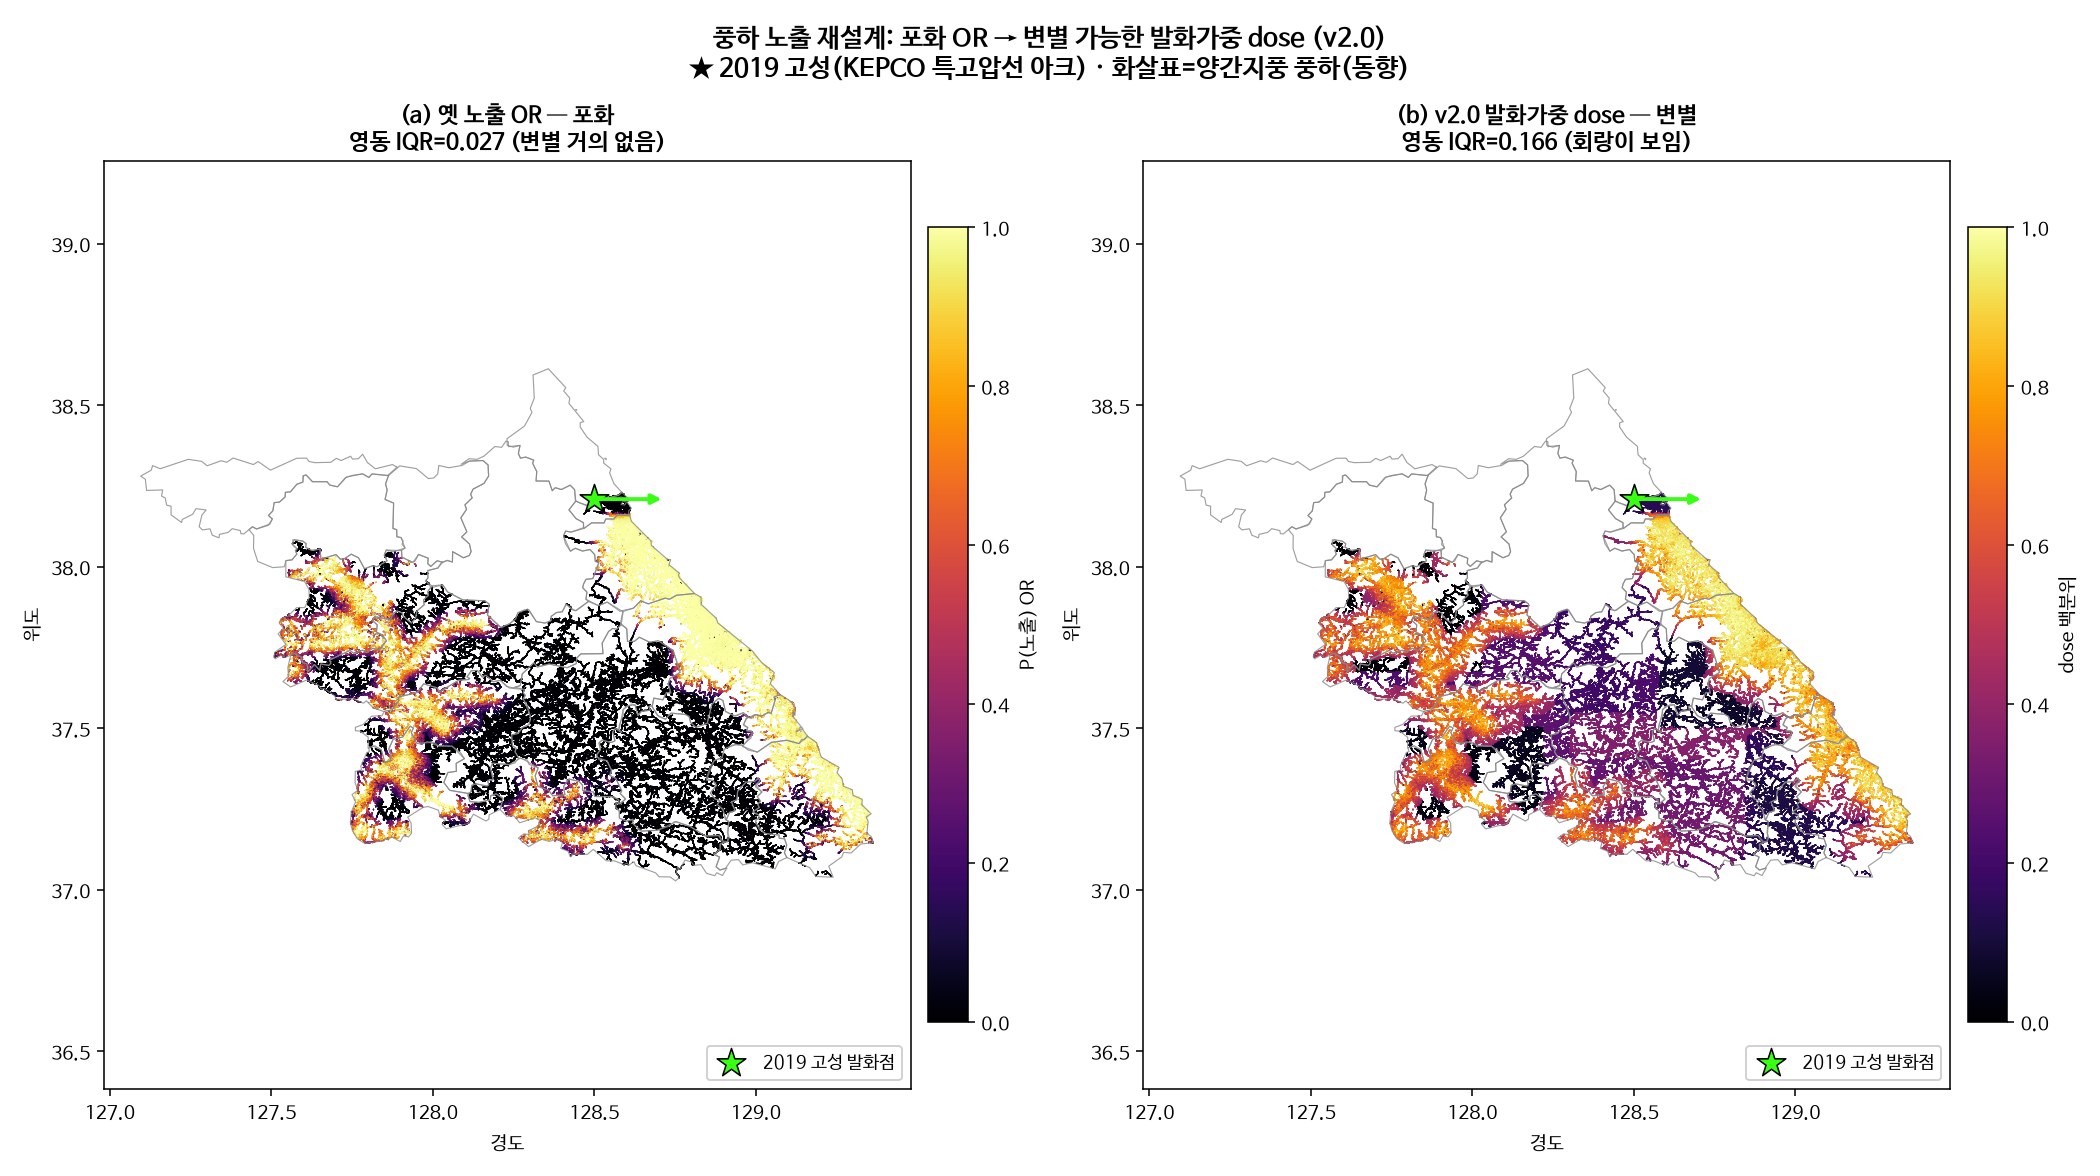
\includegraphics[width=0.92\linewidth]{fig_flagship_exposure.png}
\caption{풍하 노출 재설계. (좌) 기존 OR은 영동이 포화되어 변별이 거의 0, (우) v2.2 발화가중 도즈는
변별 그라데이션을 회복. $\bigstar$=2019 고성 발화점, 화살표=양간지풍 풍하(동향).}
\label{fig:expo}
\end{figure}

% ---------------------------------------------------------------
\subsection{5단계 — 지역율 계층 보정: 경험적 베이즈(EB)}\label{sec:eb}
% ---------------------------------------------------------------
\src{pfire/hierarchy.py}

발화점이 희소($\sim$700개)하고 일부 시군은 발화 $0\sim$소수다. 관측율을 그대로 쓰면 극단 추정으로
과적합하므로, Poisson--Gamma EB 축소로 부모 단계 평균으로 끌어당긴다(전역$\to$체제$\to$시군$\to$격자,
top-down). 지역 $g$의 관측율 $\hat\lambda_g=y_g/n_g$, 부모율 $m$·형제율 분산 $v$로 Gamma 사전을
적률추정($\alpha=m^2/v,\ \beta=m/v$)하면 사후평균은 관측율과 부모율의 볼록결합이다:
\begin{equation}
\tilde\lambda_g=\frac{y_g+\alpha}{n_g+\beta}=w_g\,\hat\lambda_g+(1-w_g)\,m,\qquad
w_g=\frac{n_g}{n_g+\beta}.
\label{eq:eb}
\end{equation}
표본 큰 지역은 관측율에 가깝고($w_g\!\to\!1$), 0발화·소표본은 부모율 $m$으로 축소된다($w_g\!\to\!0$).
전주 배율은 격자 EB율을 전역 EB율로 나눈 \emph{상대배율}(전역평균$\approx 1$)이다.

% ---------------------------------------------------------------
\subsection{6단계 — 불확실성: 베이지안 사후 + 공간 CAR}\label{sec:posterior}
% ---------------------------------------------------------------
\src{pfire/posterior.py}

\paragraph{(6a) Poisson--Gamma 켤레 사후(닫힌형).}
지역 발화수에 켤레 사전을 두면 사후가 닫힌형이라 MCMC가 불필요하다:
\begin{equation}
\lambda_g\,\big|\,y_g\ \sim\ \mathrm{Gamma}\!\big(\alpha_0+y_g,\ \beta_0+n_g\big),\qquad
\E=\tfrac{\alpha}{\beta},\quad \Var=\tfrac{\alpha}{\beta^2}.
\label{eq:pg}
\end{equation}
zero-event 지역은 $\alpha\!\to\!\alpha_0$(부모 수렴)이고 노출이 작아 $\beta$도 작으므로 \emph{사후
분산이 커진다}(불확실성 자동 표현).

\paragraph{(6b) 위험 사후예측(몬테카를로 전파).}
각 draw $r$에서 지역율 사후배율 $m^{(r)}$(전역평균$\approx 1$)을 물리 base risk에 곱해 전파한다:
\begin{equation}
R^{(r)}(p)=\clip\!\big(R_{\text{base}}(p)\cdot m^{(r)}(p),\,0,1\big),
\end{equation}
전주별 평균과 분위로 credible interval $[\,\mathrm{lo}=q_{0.05},\ \mathrm{hi}=q_{0.95}\,]$을 낸다.

\paragraph{(6c) BYM2 공간 CAR(INLA식 Laplace 근사).} \src{posterior.bym2\_spatial\_posterior}
켤레 사후는 이웃에서 정보를 빌리지 않는다. 이웃 격자 강도를 빌리도록(borrow strength) 공간 CAR로
확장한다. 격자 $i$에 대해
\begin{equation}
y_i\sim\mathrm{Poisson}\!\big(E_i\,e^{x_i}\big),\quad E_i=n_i\cdot(\text{전역율}),
\end{equation}
잠재 로그상대위험 $x$의 BYM2 prior 정밀도는 구조(ICAR)와 비구조(iid)의 보간이다:
\begin{equation}
Q_x(\tau,\phi)=\tau\big[(1-\phi)\,I+\phi\,Q_{\text{ICAR}}\big],\qquad
Q_{\text{ICAR}}=D-W+\text{jitter}\cdot I.
\label{eq:bym2Q}
\end{equation}
각 하이퍼 $(\tau,\phi)$에서 음의 로그사후
$f(x)=\sum_i(E_i e^{x_i}-y_i x_i)+\tfrac12 x^\top Q_x x$를 sparse Newton으로 최소화해 모드 $x^\star$와
Hessian $H=\mathrm{diag}(E e^{x^\star})+Q_x$를 얻고, Laplace 주변우도
\begin{equation}
\log p(y\,|\,\tau,\phi)\approx
\sum_i\!\big(y_i x_i^\star-E_i e^{x_i^\star}\big)
+\tfrac12\log|Q_x|-\tfrac12 x^{\star\top}Q_x x^\star-\tfrac12\log|H|
\label{eq:laplace}
\end{equation}
가 최대인 점을 채택한다(탐색 격자 $\tau\in\{1,3,10,30,100,300\}$, $\phi\in\{0.25,0.5,0.75,0.9\}$;
채택 $\tau{=}10,\ \phi{=}0.25$). 격자 사후는 가우시안 $x_i\sim\mathcal N(x_i^\star,(H^{-1})_{ii})$,
상대배율은 로그정규 $e^{x_i}$. 고립 격자는 iid 항만 적용해 부모(독립 Poisson--Gamma) 수준으로 폴백한다.

% ---------------------------------------------------------------
\subsection{7단계 — 임계값·보정·평가}\label{sec:eval}
% ---------------------------------------------------------------
\src{pfire/calibrate.py}

presence-only라 모델은 \emph{순위}만 내고 $0/1$ 컷은 별도로 정한다.

\paragraph{recall@top-$k$.} 위험 상위 $k\%$가 발화점-전주를 포함하는 비율(분리력 지표). 공간 블록(10\,km
GroupKFold) 홀드아웃에서 측정한다.

\paragraph{단조 보정(PAVA isotonic).} 발화점$=1$, 표본 음성$=0$으로 두고 위험점수$\to$확률을 단조
(비감소) 회귀로 보정한다(절대확률이 아닌 단조 보정값).

\paragraph{F1 민감도.} 정답 양성비율 $\rho$가 미지이므로 가정별 곡선을 보고한다. 상위 $\rho$ 분위를
양성으로 두고
\begin{equation}
\text{prec}_{\text{proxy}}=\frac{\rho\,\cdot\,\text{recall}\,\cdot\,N}{n_{\text{pred}}},\qquad
F_1=\frac{2\,\text{prec}_{\text{proxy}}\,\text{recall}}{\text{prec}_{\text{proxy}}+\text{recall}},
\quad \rho\in\{0.5,1,2,3,5,10\}\%.
\label{eq:f1}
\end{equation}

\paragraph{체제별 conformal.} 교환가능 가정만으로 유한표본 커버리지를 보장한다. 체제 $r$ 보정집합
(= train fold 발화점에 매핑된 전주)의 위험점수를 오름차순 정렬해
\begin{equation}
\tau_r=\mathrm{score}_{(\lfloor\alpha(n_r+1)\rfloor)},\qquad
\Pr\!\big(\text{새 발화점 위험}\ge\tau_r\big)\gtrsim 1-\alpha,
\label{eq:conformal}
\end{equation}
$\{p:\ \mathrm{risk}(p)\ge\tau_r\}$를 위험집합으로 둔다($\alpha=0.10\Rightarrow$ 명목 90\% 커버리지).

% =====================================================================
\section{본론 III — 학습·튜닝 절차}\label{sec:tuning}
% =====================================================================
\src{scripts/tune\_weights.py, scripts/run\_phase3.py, scripts/run\_phase1\_mvp.py}

본 시스템에는 신경망식 역전파 학습이 없다. 대신 \emph{물리식 + 데이터 구동 가중 탐색}을 쓰며, 모든
선택은 \textbf{공간 블록 교차검증(10\,km GroupKFold)}으로 누수 안전하게 결정한다(발화점은 per-pole
타깃이 아니라 fold별 집계 앵커로만 사용). 절차는 다음과 같다.

\begin{enumerate}[leftmargin=1.5em,itemsep=2pt]
\item \textbf{피처 구축}: 식\eqref{eq:decay}로 7개 발화 피처와 게이트 피처를 $[0,1]$로 정규화.
\item \textbf{게이트 계산}: 식\eqref{eq:gate}로 체제 soft 가중 $g_r(p)$, 앵커 $\mu_r$은 시군 매핑 전주의
표준화 피처 중심.
\item \textbf{전문가 가중 $w_{r,k}$ 튜닝}: 목적함수 = 공간 CV 발화점 recall@top-$\{1,2,5,10\}\%$의
가중평균(가중 $0.15/0.25/0.40/0.20$). 탐색은 \emph{LHS(Dirichlet) 랜덤 4000후보 + 좌표상승}
(passes $2{\sim}4$, step $0.05$, simplex 제약). 시작점 후보\{랜덤최선·상위평균·config baseline\} 중
최고에서 좌표상승하며 baseline-keep 가드를 둔다. provenance는 \texttt{outputs/tuned\_weights*.json}.
\item \textbf{within-목적 재튜닝(채택)}: 전역 recall은 체제 기저율(영동↑·산간↓)을 학습하는 \emph{지름길}
(Simpson 역설)에 빠질 수 있다. 이를 차단하려고 목적함수를 \emph{체제 내(within-regime) recall 동일가중
평균}으로 바꿔 4체제를 joint로 재튜닝했다. 결과: within-regime AUC $0.488\!\to\!0.560$(회랑
$0.42\!\to\!0.52$). 대가로 전역 recall@top-5\%가 $0.097\!\to\!0.071$로 하락하나, per-pole 정확성·운영
커버리지를 우선해 채택한다(표\ref{tab:weights}).
\item \textbf{$W$ 블렌드 가중 $w_s$}: 식\eqref{eq:wblend}을 $w_s\in[0,1]$ 격자 스윕, ``고성 sanity
회복 + recall 유지''를 동시 만족하는 $0.82$ 채택.
\item \textbf{풍하 노출 결합 $w$}: 식\eqref{eq:blend}을 $w$ 스윕, 5 fold-seed에서 신호$>$잡음을 확인하고
보수적 $0.25$ 채택.
\item \textbf{예산·임계값 배분}: 양성비율 $\rho=2\%$ 시 예산 $27{,}757$개. 전역 vs 체제별 배분을 공간 CV
recall로 비교해 \emph{regime\_anchor} 배분(체제별 앵커 비율) 채택(score $0.0884\!\to\!0.0926$).
\item \textbf{불확실성·커버리지}: 식\eqref{eq:pg}--\eqref{eq:laplace}로 사후, 식\eqref{eq:conformal}로
체제별 임계값. 모든 난수는 \texttt{SEED}$=20260618$로 결정적.
\end{enumerate}

% =====================================================================
\section{본론 IV — 결과}
% =====================================================================

\paragraph{공간 블록 CV 분리력.} 발화점 recall@top-$k$(10\,km 블록, 홀드아웃)는 랜덤 대비 약 2배이며
무작위-공간 격차가 $\approx 0$(낙관 편향 없음)이다(표\ref{tab:recall}). 천장(2배 수준)은 모델 실패가
아니라 \emph{앵커·피처의 구조적 한계}(매끈한 지역 피처 대 핀포인트 화재)다.

\begin{table}[H]
\centering
\caption{최종 결정 위험의 공간 블록 CV 발화점 recall@top-$k$(prevalence $2\%$, 예산 $27{,}757$).}
\label{tab:recall}
\small
\begin{tabular}{lcccc}
\toprule
지표 & top-1\% & top-2\% & top-5\% & top-10\% \\
\midrule
recall(mean) & 0.023 & 0.040 & \textbf{0.106} & \textbf{0.185} \\
랜덤 기준    & 0.010 & 0.020 & 0.050 & 0.100 \\
\bottomrule
\end{tabular}\\[2pt]
{\footnotesize 무작위-공간 격차 $=-0.0055$(랜덤 $0.1005$ vs 공간 $0.1061$, top-5\%) — 낙관 편향 없음.}
\end{table}

\paragraph{체제별 위험 분포.} 결정 양성($\rho{=}2\%$, 27{,}757개)은 영동 $2.01\%$(전주 305{,}589),
영서 $2.38\%$(662{,}308), 산간 $1.40\%$(419{,}934)로 배분되어 인간발화 중심 영서가 다수를 차지하되
영동·회랑의 강풍 위험이 백분위로 보존된다.

\paragraph{풍하 노출 v2.2.} 국지정규화로 영동 내 변별 IQR이 $0.166\!\to\!0.290$로 회복되고
(그림\ref{fig:expo}), 식\eqref{eq:blend} 결합 시 공간 CV recall이 일관되게 상승한다.

\paragraph{설비원인 검증 + asset ablation.} 핵심 novelty(``전주=전력설비 자산을 발화원으로 모델'')를
두 실험으로 정직하게 검증했다(표\ref{tab:asset}). 공정 LOGO ablation에서 설비 근접 피처는 거의
중립이지만(top-5\% $+0.011$), \emph{원인별} recall에서 설비전기 화재는 인간발화보다 더 잘 회수된다
(top-10\% $0.167$ vs $0.151$). 즉 위험맵은 한전 관심사인 설비화재에 정렬하나, 그것이 단일 피처 기여라기
보다 공유 물리에 흡수된 결과다. 설비 표본 $n{=}18$로 희소하여 \emph{방향·메커니즘}으로만 해석한다.

\begin{table}[H]
\centering
\caption{(좌) asset ablation recall, (우) 원인별 recall.}
\label{tab:asset}
\small
\begin{tabular}{lcc@{\hskip 1.2cm}lcc}
\toprule
arm & top-5\% & top-10\% & 원인 & top-5\% & top-10\% \\
\midrule
blind          & 0.092 & \textbf{0.189} & 설비전기($n{=}18$)  & \textbf{0.111} & \textbf{0.167} \\
aware(+송전선)  & \textbf{0.103} & 0.183 & 인간($n{=}476$)     & 0.079 & 0.151 \\
\bottomrule
\end{tabular}
\end{table}

\paragraph{불확실성·커버리지.} 체제별 conformal은 명목 90\%에 정확히 보정된다(전체 $0.902$, 영동
$0.907$, 영서 $0.900$, 산간 $0.903$). credible 밴드 단독은 보수적(과커버 $1.0$)이다. BYM2 공간 사후는
독립 Poisson--Gamma 대비 이웃에서 강도를 빌려 공간 자기상관을 강화하고(Moran's $I$ $0.082\!\to\!0.112$),
소표본 시군(예: 태백)의 배율을 부모 쪽으로 끌어올린다($\Delta\!\approx\!+0.30$, watch 대상). 운영
우선순위(``위험하지만 불확실'') 전주는 $111{,}462$개로 능동 라벨 수집 후보가 된다.

\begin{figure}[H]
\centering

\includegraphics[width=0.78\linewidth]{fig9_coverage.png}
\caption{체제별 명목 90\% 대 실측 커버리지(공간블록 누수안전 홀드아웃). conformal이 합격선
($\approx$90\%)에 정렬, credible 밴드는 보수적.}
\label{fig:cov}
\end{figure}

\paragraph{2019 고성 사례(간판 시나리오).} 발화점(서)에서 양간지풍 풍하(동)로 흉터가 번지고, 전주
위험 점수도 같은 서$\to$동 축으로 분포해 발화·확산 시나리오와 정합한다(그림\ref{fig:goseong}).

\begin{figure}[H]
\centering

\includegraphics[width=0.82\linewidth]{fig_goseong_corridor.png}
\caption{2019 고성--속초 산불 케이스 — 발화점·양간지풍 풍하 방향·전주 위험 점수의 정합(회랑 체제).}
\label{fig:goseong}
\end{figure}

% =====================================================================
\section{결론}
% =====================================================================

\subsection{요약}
MOSAIC은 라벨 없는(presence-only) 전주 산불 위험을 (i)~물리적 곱셈 분해 $h=I\cdot S\cdot W$로
해석 가능하게 구성하고, (ii)~발화 메커니즘이 다른 4개 체제를 soft 게이트 혼합전문가로 부분 풀링하며,
(iii)~포화되던 풍하 노출을 변별 가능한 발화가중 도즈로 재설계해 결정에 결합하고, (iv)~경험적 베이즈와
BYM2 공간 사후로 불확실성을, 체제별 conformal로 명목 90\% 커버리지를 보장한다. 공간 블록 CV에서
recall이 랜덤의 약 2배이고 무작위-공간 격차가 $\approx 0$이라 \emph{낙관 편향이 없으며}, 발화점을
어디서도 per-pole 학습 라벨로 쓰지 않아 누수가 차단된다.

\subsection{한계(정직한 노출)}
산출물은 \emph{절대 확률}이 아니라 상대 순위다(presence-only). $0/1$ 컷은 양성비율 가정에 의존하므로
F1 민감도 곡선으로 투명하게 보고한다. 검증 앵커가 인간발화 위주라 모든 정량은 \emph{프록시} 기준이며
한전 실타깃과의 정렬은 미지다. within-regime 신호가 원래 약할 수 있어(체제 내 AUC $\approx 0.5$),
within-목적 튜닝의 1차 가치는 ``정직한 추정''이며 무리한 끌어올림은 과적합 위험이 있다. 시군구 단위로
더 잘게 쪼개는 실험은 $\sim$700개 앵커로 일반화되지 않아(과세분) 채택하지 않았고, 토지피복은 산림
거리와 일부 중복된다 --- 이는 모델 결함이 아니라 \emph{구조적 정보병목}의 노출이다.

\subsection{활용 방안}
한전 실무에는 (i)~고위험일 풍하 고노출 전주의 \emph{일별 순시 우선순위}, (ii)~시즌 상위 전주의
\emph{절연 보강·수목 제거(vegetation management)} 대상 선정, (iii)~``위험하지만 불확실''($111{,}462$개)
전주의 \emph{현장 확인 우선}(능동 라벨 수집)으로 쓰인다. 향후 FFAS(산림청 산불발생대장, 강원 4{,}851건)의
\emph{발화시각}을 활용한 케이스-크로스오버 검증으로 기상 피처의 시간축 분리력을 캘리브레이션하면 정성
점수와 운영 신뢰도를 함께 높일 수 있다. 같은 패러다임으로 운영되는 해외 전력사(예: PG\&E)의 배전선
발화 감소 사례가 본 시스템의 가치를 뒷받침한다.

% =====================================================================
\appendix
\section{상수 요약}
\src{pfire/config.py}
\begin{center}
\small
\begin{tabular}{lll}
\toprule
파라미터 & 값 & 의미 \\
\midrule
거리 감쇠 scale & 100/300/1500/3000\,m & 산림/도로/송전선/변전소(식\ref{eq:decay}) \\
게이트 온도 $\tau$ & 0.6 & 작을수록 하드 게이트(식\ref{eq:gate}) \\
$W$ 블렌드 $w_s$ & 0.82 & 시즌극값 : 일별동역학(식\ref{eq:wblend}) \\
ISI/FFMC/양간 성분 & 0.05 / 0.75 / 0.20 & 일별 $W$ 결합(식\ref{eq:wdaily}) \\
고-ISI / 고-FFMC 임계 & 10.0 / 90.0 & 관측소 일별 $q90$ 정합 \\
LWR 상한 & 8.0 & Anderson 길이/폭비 cap(식\ref{eq:lwr}) \\
$W_\perp,\ L_{\text{back}}$ & 0.35 / 0.35\,km & 횡풍/풍상 스케일(식\ref{eq:dose}) \\
국지정규화 셀 & 4.0\,km & 영동 배경 제거(식\ref{eq:dose01}) \\
노출 결합 $w$ & 0.25 & $R'=1-(1-R)(1-w\,e)$(식\ref{eq:blend}) \\
확산 컷오프 / 발화후보 & 5.0\,km / 상위 2\%(상한 8000) & 2019 고성 스케일 \\
양간 풍향 prior & $270^\circ\!\pm\!20^\circ$ & 영동·회랑 서풍 푄 \\
conformal $\alpha$ & 0.10 & 명목 90\% 커버리지(식\ref{eq:conformal}) \\
BYM2 $(\tau,\phi)$ 채택 & $(10,\ 0.25)$ & 정밀도·구조비(식\ref{eq:bym2Q}) \\
SEED & 20260618 & 전 과정 결정성 \\
\bottomrule
\end{tabular}
\end{center}

\vspace{6pt}\hrule\vspace{4pt}
{\footnotesize 모든 식은 \texttt{pfire/} 모듈 구현과 일치하며, 발화점은 어디서도 per-pole 학습
라벨이 아니라 \emph{지역 집계 앵커 · 검증 · 임계값}으로만 쓰인다(누수 안전).}

% =====================================================================
\begin{thebibliography}{9}\small
\bibitem{kiryo} R.~Kiryo et al., ``Positive-Unlabeled Learning with Non-Negative Risk Estimator,'' \emph{NeurIPS}, 2017.
\bibitem{jacobs} R.~Jacobs et al., ``Adaptive Mixtures of Local Experts,'' \emph{Neural Computation}, 1991.
\bibitem{anderson} H.~Anderson, ``Predicting Wind-Driven Wildland Fire Size and Shape,'' \emph{USDA FS} INT-305, 1983.
\bibitem{ager} A.~Ager et al., ``Wildfire exposure and source--sink relationships,'' \emph{Forest Ecol. Manage.}, 2012.
\bibitem{finney} M.~Finney, ``Fire growth using minimum travel time methods,'' \emph{Can. J. For. Res.}, 2002.
\bibitem{riebler} A.~Riebler et al., ``An intuitive Bayesian spatial model for disease mapping (BYM2),'' \emph{Stat. Methods Med. Res.}, 2016.
\bibitem{rue} H.~Rue et al., ``Approximate Bayesian inference (INLA),'' \emph{J.\ R.\ Stat.\ Soc.\ B}, 2009.
\bibitem{getis} A.~Getis, J.~Ord, ``The Analysis of Spatial Association,'' \emph{Geographical Analysis}, 1992.
\bibitem{ploton} P.~Ploton et al., ``Spatial validation reveals poor predictive performance,'' \emph{Nature Comm.}, 2020.
\bibitem{angelopoulos} A.~Angelopoulos, S.~Bates, ``A Gentle Introduction to Conformal Prediction,'' arXiv:2107.07511, 2021.
\end{thebibliography}

\end{document}
